\section*{\LARGE Appendix}
\counterwithin{figure}{subsection}
\renewcommand{\thefigure}{\thesubsection.\alph{figure}}

\section{Methodology}


\subsection{Scaling with national accounts}
\label{aux:scaling}

Households' propensities to consume are the first term in \cref{eq:TIR}. Taxable consumption includes all monetary expenditure, excluding rents, which are not subject to consumption taxes. Moreover, loan repayments are considered as savings, not consumption.

\[ prop_i = \frac{hmc_i-rents_i}{dhi_i} \]
where $hmc$ is household monetary consumption, $rents$ is household expenditure in rentals, $dhi$ is disposable income of household.

Disposable income is the amount of money that households have available for spending after income taxes, social security contributions, and transfers have been accounted for.

After some preprocessing on the data (equivalization, bottom-coding), propensities to consume are scaled according to national accounts data. In order to do a international comparison, micro-data is transformed to reflect the amounts of consumption and income at the national level. Conceptually, this means that micro-data are used to get the shape of consumption (its relative distribution with income), while the total levels of income and consumption are put in accordance with national accounts.

We apply a scaling factor on propensities to consume.

\[ scaled\ prop_{c,y,i} = scaling_{c,y} \cdot prop_{c,y,i} \]

\[ scaling_{c,y} = \frac{CH-R}{I-R_{imputed}} \cdot \frac{\sum_i dhi_i}{\sum_i hmc_i-hmchous_i } \]
where:
\begin{itemize}
\item $CH$ is final consumption expenditure of households\footnote{When this figure was not available, we used expenditure and income of households and non-profit institutions serving households.}
\item $I$ is gross disposable income of households
\end{itemize}

In national accounts, services of housing that owners produce for themselves are included in both the consumption expenditure and the income of households. We thus remove those terms from the scaling factor of propensities to consume. For some countries however, information on imputed rentals was missing, so this term was omitted.

These national accounts ratios are stored in a Stata data file, and scaling factors are computed after the preprocessing.

We are now able to compute the tax ratio on each household $i$ in country $c$ at year $y$, that is
\[ TIR_i = \tau_{c,y} \cdot scaled\ prop_{c,y,i} = \underbrace{\tau_{c,y} \cdot \frac{CH-R}{I-R_{imputed}}}_{macro\ data} \cdot \underbrace{\frac{\sum_i dhi_i}{\sum_i hmc_i-hmchous_i } \cdot prop_i}_{micro\ data}  \]

\subsection{Definition of effective tax rate}

We define tax rates implicitly: instead of using official statutory rates that do not reflect the average rate at which households' consumption is taxed, we use tax revenue and consumption data from national accounts. For each country-year, we compute the ratio between consumption taxes revenue and the amount of taxable consumption. This defines the average effective tax rate on consumption paid by households.

We rely on previous research on implicit tax rates (see \cref{appendix_itrc}), and try to improve existing definitions by defining the effective tax rate as follows:
\[ \tau_{c,y} = \frac{consumption\ taxes\ revenue}{C - CGW - R} \]
where $consumption\ taxes\ revenue$ includes all revenue from consumption taxes, including value-added-taxes (or sales taxes if applicable), excise taxes, taxes on specific services, etc. $C$ is the total final consumption expenditure (private consumption and consumption of general government). $CGW$ is the amount of wages of employees paid by general government, and $R = R_{actual} + R_{imputed} =$ are actual and imputed rentals for housing.

It is important to note that the ``final consumption expenditure of households'' includes actual rentals that tenants are paying and imputed rentals that occupying owners are paying to themselves. We need to remove this from the denominator, as it generates no tax revenue.

The government does not purchase its whole consumption. In order to account for the share of its consumption that is self-produced (and thus does not generate tax revenue), we remove the term $CGW$ from the denominator, as per \cite{mendoza1994effective}.

For each country-year, we compute tax rates according to the three available definitions. When some numbers are missing, we impute rates with a regression model based on other tax rates (see \cref{appendix_itrc}).


\subsection{Consumption imputation model}
\label{app:imputation_model}

We use a generalized linear model in order to impute consumption data according to households characteristics. The key issue here is that consumption data will have to be imputed on whole datasets for which there is no observation on expenditure. Therefore, it is necessary to design a model that can be calibrated on some countries and used on others.

In order to achieve that, we apply medianization to all monetary variables (including income, consumption and value of housing). That is, all monetary variables are expressed in proportion of their median values in the dataset. The \textbf{medianized disposable income} is thus:
\[ \widehat{income}_i = \frac{income_i}{\text{median}_{c,y}(income_i)} \]

The underlying assumption is that the relations between medianized consumption and medianized income are similar in every country, account taken of other individuals determinants. In order to reduce the heterogeneity of the different countries, we remove from the training sample a few countries whose income distributions are the most extreme. That is, countries with a high degree of income inequality or with very low median income, compared to the rest of the sample. The list of countries used in the regression are listed in \cref{A-datasets}. We nonetheless apply the imputation model to every country, whether they have been used to calibrate the model or not.

We design two nested models, depending on the information available in the dataset. The first one is a generalized linear model where dependent variables are the medianized disposable income of the household, a few socio-demographic determinants (number of members in household and conjugal status of head), and a binary variable indicating whether the household is under the monetary poverty threshold. This threshold is defined as 60\% of the median equivalized income. Therefore, a household is under the poverty threshold if its medianized disposable income is under 0.6. This indicator has been added in order to account for the fact that, for lowest incomes, levels of consumption tend to be less correlated (even not correlated) with income [référence à ajouter]. Therefore, this indicator allows to account for different consumption patterns of poor households.
\begin{equation}
\label{equ:mod1}
    \log(\widehat{hmc}) = \alpha_0 +\beta_0\log(\widehat{dhi})
    + \mathbbm{1}_{pov}\cdot\left[\alpha_1 + \beta_1\log(\widehat{dhi})\right] + \Gamma^\intercal X + \epsilon
    \tag{mod.\ 1}
\end{equation}

In the second nested model, we add some socio-demographic determinants (number of people aged 65 or older, number of wage income-earners in household, housing ownership status). Moreover, we add another monetary variable that is the total imputed or effective cost of housing. This amount may correspond to actual money spent by the household in rentals, or to non-monetary consumption for housing services (e.g.\ imputed rents for occupying owners). This variable is much more widely available in households surveys than total consumption, and is a good proxy of the standard of living of the household. Therefore, it carries valuable information on the amount of consumption of the household. The second model is thus:
\begin{equation}
\label{equ:mod2}
    \log(\widehat{hmc}) = \alpha_0 +\beta_0\log(\widehat{dhi})
    + \mathbbm{1}_{pov}\cdot\left[\alpha_1 + \beta_1\log(\widehat{dhi})\right]
    + \delta\log(\widehat{housing}) + \Theta^\intercal Y + \epsilon
    \tag{mod.\ 2}
\end{equation}

With this regression model, we impute medianized values of the households' monetary consumption. It is then scaled with national accounts data in order to be comparable with observed values, according to section \ref{subsub:prop}.

\section{Robustness checks}
\subsection{Different definitions of effective tax rate}
\label{appendix_itrc}

\begin{figure}[!ht]
\centering
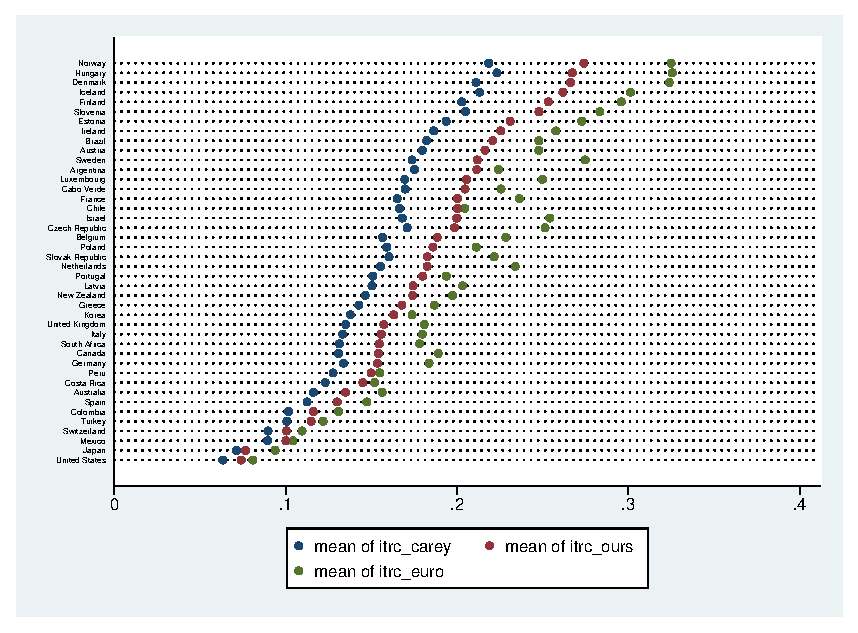
\includegraphics[width=0.9\textwidth]{images/18-09_itrc_comparison}
\caption{Mean of implicit tax rates on consumption for each country.}
\label{fig:itrc_comparison}  
\end{figure}

There are three main definitions for computing implicit effective tax rates on consumption in the economic literature, as described in \cite{euro2016taxation, mendoza1994effective, carey2000average}. We draw on those works in order to propose the following definition:
\[ \tau_{c,y} = \frac{consumption\ taxes\ revenue}{C - CGW - R } \]
where $consumption\ taxes\ revenue$ includes all revenue from consumption taxes, including value-added-taxes (or sales taxes if applicable), excise taxes, taxes on specific services, etc. $C = CP + CG$ is the total final consumption expenditure (private consumption and consumption of general government). $CGW$ is the amount of wages of employees paid by general government, and $R = R_{actual} + R_{imputed} =$ are actual and imputed rentals for housing.

The different possible definitions of implicit tax rates rely on different definitions of the taxable consumption. For example, the definition in \cite{euro2016taxation} relies on a narrower taxable basis, constituted only of private consumption
\begin{equation}
    \label{itrc_euro}
    \tau_{c,y} = \frac{consumption\ taxes\ revenue}{CP}
\end{equation}
while the definition in \cite{carey2000average} considers a broader definition, by taking all consumption
\begin{equation}
    \label{itrc_carey}
    \tau_{c,y} = \frac{consumption\ taxes\ revenue}{C}
\end{equation}

The choice of removing or not rents from the denominator depends on the definition of taxable consumption in micro-data. Since we account for the fact that rents are not subject to consumption taxes by removing rents from the micro-data on consumption, we subtract rents from the denominator of the implicit tax rate. If we do the same for the two alternative definitions described earlier, our definition of implicit tax rates on consumption is thus structurally bounded above by the tax rate under definition \eqref{itrc_euro} and below by that under definition \eqref{itrc_carey} (see \cref{fig:itrc_comparison}). These alternative definitions can be used to produce robustness checks.

\subsection{Estimated regressivity is mitigated when taking rents into account}
\label{sec:rents}
\begin{figure}[!h]
\centering
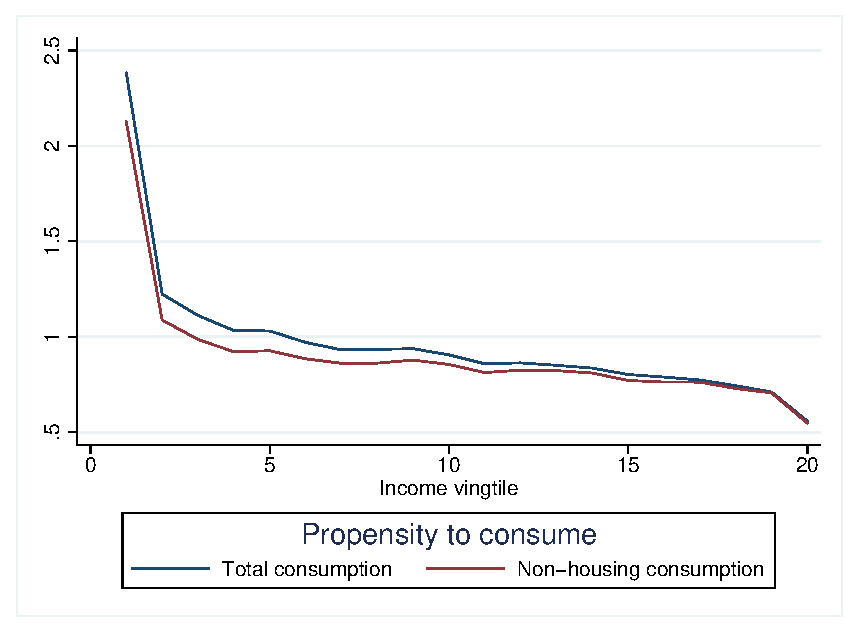
\includegraphics[height=0.4\textheight]{images/18-11-18_total_nonrent_propensity_fr10}
\caption{Rents represent a higher share of consumption at the bottom of the income distribution (France 2010)}
\label{fig:total_nonrent}  
\end{figure}

Our method allows to account for the fact that housing rentals are not subject to consumption taxes. They are an important part of households' consumption, and they represent a higher share of consumption for poorer households (\cref{fig:total_nonrent}). As a result, the downward slope of propensities to consume are less pronounced when rents are removed from the total amount of consumption. Therefore, we can conclude that micro-simulation methods which apply tax rates on the whole consumption (rent or not) are slightly overestimating the regressivity of consumption taxes.

In order to maximize our coverage of countries and years, we also define another version of the effective tax rate, where actual rentals are not removed from private consumption at the denominator. This definition will be used when micro-data on consumption is not separable between rentals and the rest of the consumption. This smaller rate will be applied on a bigger amount of consumption.
\[ \tau_{wr}= \frac{consumption\ taxes\ revenue}{CP - R_{imputed} + CG - CGW}\]

As shown in \cref{fig:kakrent}, estimated regressivity is reduced when rents are taken into account, and removed from the amount of consumption: the absolute value of the Kakwani index of regressivity can be reduced by up to 20\% for some countries.

\begin{figure}
\centering
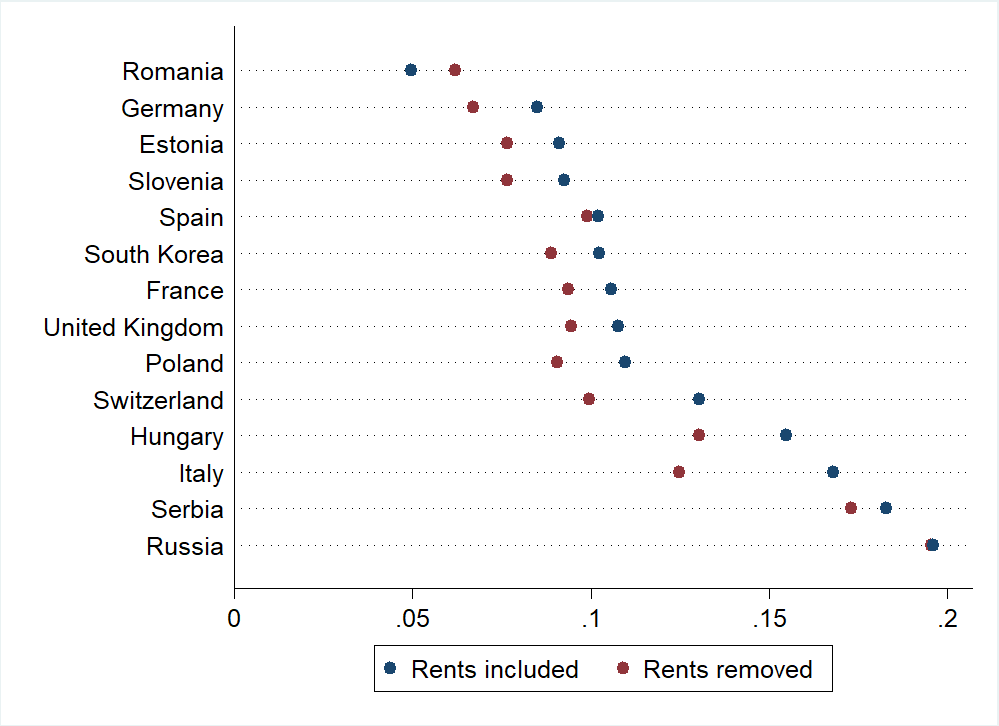
\includegraphics[width=0.9\textwidth]{images/18-03-18_kak_kak_wor_mean}
\caption{\label{fig:kakrent} Mean value of Kakwani index whether taxable consumption includes rentals}
\end{figure}

\subsection{Progressive consumption tax rates: test of the bundle effect}
\label{sec:diff_rates}  
Many countries enforce reduced VAT rates for some goods, either in order to boost some economic sectors or to lighten the amount of consumption taxes paid by least affluent households. On the other hand, some goods are more heavily taxed, such as oil or alcohol.

These variations on statutory tax rates can affect the overall progressivity of the tax, as the baskets of goods are different at one point or another of the income distribution. As a robustness check, we design two scenarios, where the effective tax rate is increasing with income. These situations would occur if tax rates had been specifically designed to make consumption taxes more progressive, as it is generally the case. These scenarios introduce a deviation from the median effective tax rate that depends linearly on the percentile of income. In the intermediate scenario, the first percentile of income enjoys an 0.5 percentage points lower effective tax rate than the median household, while the last percentile faces a 0.5 points higher tax rate, so that there is a 1 percentage point difference between the effective tax rate paid by poorest households and richest households. We also provide an extreme scenario where the gap between effective consumption tax rates at both ends is 2 percentage points. Those gaps are in accordance with national case studies that compute effective tax rates depending on income. %TODO : ajouter référence sur les effective tax rates selon décile

We show in \cref{fig:diff_rates} the distribution of tax-to-income ratios by percentiles of income. This allows to compare different situations, from the least progressive to the more progressive. In the first situation, we assume that all goods and services (including housing) would be taxed at the same effective tax rates for all households. The regressive pattern then comes exclusively from the propensity to consume. In the second curve, consumption taxes are applied only on non-housing consumption, which mitigates the regressive pattern (as seen in \cref{sec:rents}). The third and fourth curves introduce progressive consumption taxes according to the intermediate and extreme scenarios.

The curves are very close to one another: this confirms that the ` propensity to consume'' effect is the first order effect. Indeed, simulating an aggregated amount of consumption for each household allows to capture most of the regressivity of consumption taxes. When added the fact that housing consumption is not uniformly distributed, a uniform effective tax rate is even closer to the two scenarios of progressive tax rates.

Eventually, the first and last curves yield upper and lower bounds for the regressivity of consumption taxes. Indeed, we know that using the same effective tax rate for every household, and not taking into account the fact that housing is not subject to consumption taxes actually yields an overestimation of the regressivity of consumption taxes. On the other hand, when we take housing rentals into account and we apply a strong progressivity to effective consumption tax rates, we know that this yields a lower bound of the regressive effect. We can observe that even in the extreme scenario, tax-to-income ratios still present a strong regressive pattern.

The same can be said when looking at measures of redistribution and inequality. \Cref{fig:sum_diff_rates} shows that a constant effective tax rate on whole consumption produces the highest post-tax Gini index (overestimating the eventual income inequality). Adding the information on rent captures most of the difference between the latter and both progressive scenarios. In every case, we observe that all those measures of post-tax income inequality are much closer to one another than to the inequality of disposable income. Qualitatively, the anti-redistributive effect stays significant, and the first and simplest measure provides a quite tight upper bound.

\begin{figure}[!ht]
\centering
\includegraphics[height=0.45\textheight]{"images/20-01 diff_rates"}
\caption{Tax-to-income ratios for France 2010. Medium scenario: 1 pct point difference between effective consumption tax rates of the richest and the least affluent. Extreme scenario: 2 pct points difference}
\label{fig:diff_rates}  
\end{figure}

\begin{figure}[!h]
\centering
\includegraphics[width=0.90\textwidth]{"images/19-11_fr10_sum_diff_rates"}
\caption{Gini indices of income inequality for France 2010. Medium scenario: 1 pct point difference between effective consumption tax rates of the richest and the least affluent. Extreme scenario: 2 pct points difference}
\label{fig:sum_diff_rates}  
\end{figure}

\subsection{Imputation error on consumption depending on the model}
\label{sec:compare_models}
\Cref{fig:compare_models} shows the R2 coefficient for 57 countries-years where imputed and observed values of consumption can be compared. Out of the 57 country-years for which we impute consumption both with \eqref{equ:mod1} and \eqref{equ:mod2}, we observe that model 2 increases the explained variance for 54 of them. On average, it is increased by 33\%, as measured by the R2 coefficient. Overall, the R2 coefficient for model 2 is 0.45 on average, being larger than 0.36 for 75\% of country-years, and larger than 0.56 for a quarter of our observations.

This shows that the independent variable ``cost of housing'', which is the main difference between the two models, provides significant additional information for the imputation of the households' consumption.

\begin{figure}[!h]
\centering
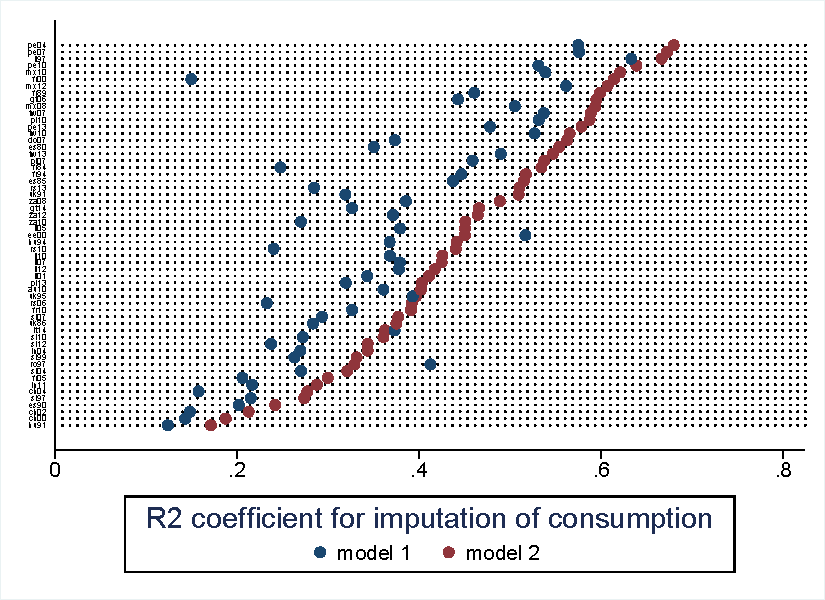
\includegraphics[width=\textwidth]{images/19-04-05_R2_compare_models}
\caption{Explained variance in the two models for various countries}
\label{fig:compare_models}  
\end{figure}

\section{Decomposition of redistributive effect}

\subsection{Vertical and horizontal redistribution}
\label{sec:decomposition}
Effective redistribution can be decomposed into vertical redistribution, measured by the Reynolds-Smolensky index ($RS$), and horizontal redistribution, measured by the reranking index ($Re$):
\begin{equation}
 \label{equ:g_diff}
    \Delta G = G_{dhi} - G_{dhi-tax}  = RS - Re
\end{equation}

Vertical redistribution relates to the amount of tax that is distributed in a progressive or regressive way related to income. A measure of vertical redistribution, the Reynolds-Smolensky index, is defined as follows [reference à ajouter]:
\[ RS = G_{dhi} - C(dhi-tax, dhi) \]
where $G_{dhi}$ is the Gini index of the pre-tax income, while $C(dhi-tax,dhi)$ is the concentration index of the post-tax income ordered on the pre-tax income. This term is thus relatively close to the Gini index of the post-tax income.

Horizontal redistribution is the amount of redistribution that is orthogonal to the distribution of income. The reranking index of horizontal redistribution is a measure of the amount of redistribution that is not due to the regressivity of the tax, but rather an inequality that is created between individuals in the same range of income. It is defined as follows:
\[ Re = G_{dhi-tax} - C(dhi-tax,dhi) \]

By definition, the reranking $Re$ is non-negative, so by \cref{equ:g_diff} the Reynolds-Smolensky index is an upper bound for effective redistribution, and it is a measure of the maximum reachable redistribution if no reranking was entailed by consumption taxes. In our case, if redistribution is negative, then the RS index is a lower bound for the anti-redistributive effect (in absolute value). The rise in income inequality due to taxes is thus the sum of the vertical anti-redistribution (due to the regressive pattern) and the reranking due to the variation in propensities to consume between households of same levels of income. In practice, the Reynolds-Smolensky index is close to the difference in Gini coefficients (see \cref{fig:reranking}): the reranking generally accounts for less than 20\% of the redistributive impact. 

\begin{figure}
    \centering
    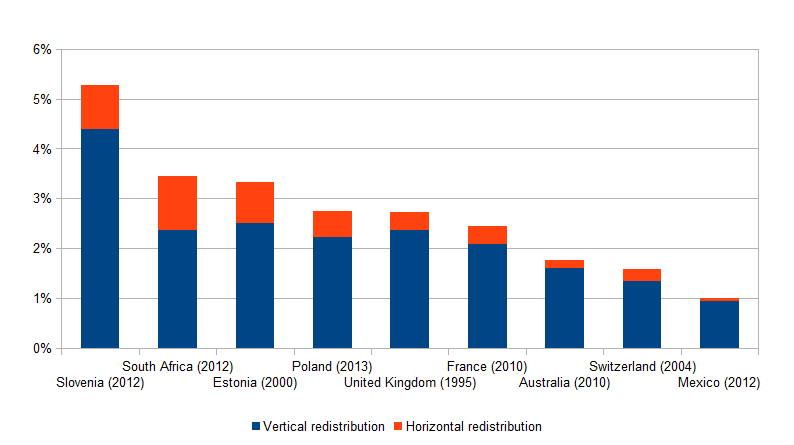
\includegraphics[width=\textwidth]{images/19-02_decomposition_effective_redistribution}
    \caption{Decomposition of redistributive effect}
    \label{fig:reranking}
\end{figure}


\subsection{Kakwani indices of regressivity}
\label{sec:kakwani}

We have seen in \cref{equ:decomp_RS} that the vertical redistribution operated by consumption taxes can be viewed as the product of two independent terms: the regressivity, a micro-level term linked to propensities to consume decreasing with income, and the rate of consumption taxes, a macro-level term.

We use the Kakwani index as an index of regressivity of consumption taxes. This indicator is a measure of how concentrated taxes are on one end of the income distribution or the other. It is equal to the difference between the concentration index of the tax relatively to (pre-tax) income and the Gini coefficient of the income [référence à ajouter]. Namely:
\[ Kakwani(tax, dhi) = C(tax,dhi) - Gini(dhi) \]

The concentration index $C(tax,dhi)$ is a measure of how much the distribution of the tax payments is skewed towards highest incomes. The range of its values is [-1;1], -1 indicating that all the tax payments are concentrated on the one poorest individual, while 1 indicates that all the tax payments are concentrated on the richest individual. The computation of this concentration index does not take into account the level of initial income inequality. By substracting the Gini index of income, the Kakwani index provides simple information, based on its sign: if the Kakwani index is positive, it means that the tax payments are more heavily concentrated towards the highest percentiles of income than income itself, meaning that the tax is progressive. On the contrary, if the Kakwani index is negative, then the distribution of tax payments is less skewed to the right than the distribution of income, meaning that the tax is regressive. We are thus expecting negative Kakwani indices.

For one fixed tax rate, we can make assumptions on the Kakwani index and thus have a range of possible RS index values. When the Kakwani indices are derived from imputed consumption values, this will be useful to provide lower and upper bounds on the possible RS values.

We compute the Kakwani index for all the datasets where consumption data is available (i.e.\ 77 country-years), the results are summed up in \cref{fig:kakwani_boxplot}. Approximately half of Kakwani indices lie between -0.10 and -0.15, while almost all of them lie between -0.05 and -0.20.
\begin{figure}
    \centering
    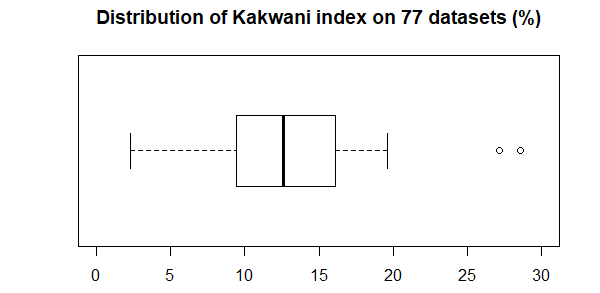
\includegraphics{images/boxplot_kakwani.png}
    \caption{Boxplot of the Kakwani indices}
    \label{fig:kakwani_boxplot}
\end{figure}

Based on the different tax rates that we have computed earlier, we are now able to frame the possible values of the RS index. As summed up in \cref{fig:RS_scenarii}, most values for the Reynolds-Smolensky index will lie between -0.02 and -0.08.
\begin{figure}
	\centering
	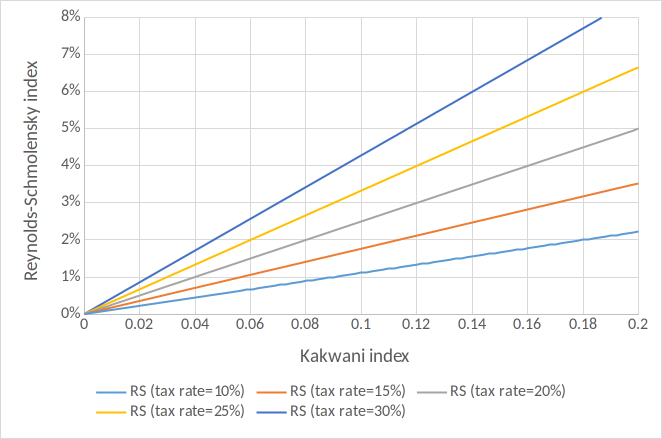
\includegraphics[scale=0.8]{images/18-12_RS_scenarii}
	\caption{Value of Reynolds-Smolensky index depending on tax rate and Kakwani index}
	\label{fig:RS_scenarii}
\end{figure}

\section{Country and years coverage}
\label{A-datasets}
We select a total of \textbf{216} LIS datasets. 

In \cref{tab:datasets}, countries marked with an \textbf{(R)} are used in the regression pool. For years marked with an *, information on rents is missing.

\begin{tabularx}{\textwidth}{lXX}
        \caption{Country and years used in the study} \\
\hline
Country            & Years with observed data                       & Years with imputed data                                       \\ \hline
Australia \textbf{(R)}      & 2010*                                          & 1989, 1995, 2001, 2003, 2008                                  \\
Austria            &                                                & 1994, 1995, 1997, 2000, 2004, 2007, 2010, 2013                \\
Belgium            &                                                & 1992, 1995, 1997*, 2000                                       \\
Brazil             &                                                & 2006, 2009, 2011, 2013                                        \\
Colombia           &                                                & 2007, 2010, 2013                                              \\
Czech Republic     &                                                & 2004, 2007, 2010, 2013                                        \\
Denmark            &                                                & 1987*, 1992, 2000, 2004, 2007*, 2010*, 2013*                  \\
Dominican Republic & 2007                                           &                                                               \\
Estonia            & 2000                                           & 2004, 2007, 2010, 2013                                        \\
Finland            &                                                & 1987*, 1991, 1995*, 2000*, 2004*, 2007*, 2010*, 2013*         \\
France \textbf{(R)}         & 1984, 1989, 1994, 2000, 2005, 2010             &                                                               \\
Germany            &                                                & 1984, 1989, 1994, 2000, 2004, 2007, 2010, 2013                \\
Greece             &                                                & 2004, 2007, 2010, 2013                                        \\
Guatemala          & 2006, 2014                                     & 2011                                                          \\
Hungary \textbf{(R)}        & 1991, 1994, 1999, 2005, 2007, 2009, 2012       &                                                               \\
Iceland            &                                                & 2004, 2007, 2010                                              \\
India              & 2004, 2011                                     &                                                               \\
Ireland            &                                                & 1994, 1995, 1996, 2000, 2004, 2007, 2010                      \\
Israel             & 2001, 2005, 2007, 2010, 2012                   & 1979*                                                         \\
Italy \textbf{(R)}          & 1995*, 1998*, 2000*, 2004*, 2008*, 2010*, 2014 & 1986*, 1987, 1989, 1991, 1993                                 \\
Japan              &                                                & 2008                                                          \\
Luxembourg         &                                                & 1991, 1994, 1997, 2000, 2007, 2010, 2013                      \\
Mexico             & 2008, 2010, 2012                               & 1984*, 1989*, 1992*, 1994*, 1996*, 1998*, 2000*, 2002*, 2004* \\
Netherlands        &                                                & 1983*, 1987, 2004, 2007, 2010, 2013                           \\
Norway             &                                                & 1979*                                                         \\
Panama             &                                                & 2010, 2013                                                    \\
Paraguay           &                                                & 2010, 2013                                                    \\
Peru               & 2004, 2007, 2010, 2013                         &                                                               \\
Poland \textbf{(R)}         & 2007, 2010, 2013                               & 1986*, 1995*, 1999*, 2004*                                    \\
Russia             & 2000, 2004, 2007, 2010, 2013                   &                                                               \\
Serbia             & 2006, 2010, 2013                               &                                                               \\
Slovakia           &                                                & 2004, 2007, 2010, 2013                                        \\
Slovenia \textbf{(R)}       & 1997, 1999, 2004, 2007, 2010, 2012             &                                                               \\
Spain \textbf{(R)}          & 1980, 1990                                     & 1995, 2000, 2004, 2007, 2010, 2013                            \\
Sweden             &                                                & 2000, 2005                                                    \\
Switzerland        &                                                & 1982*, 1992, 2007, 2010, 2013                                 \\
Taiwan \textbf{(R)}         & 1981, 1986, 1991, 2007, 2010, 2013             & 1995*, 1997*, 2000*, 2005*                                    \\
United Kingdom \textbf{(R)} & 1986, 1991, 1995                               & 1994, 1999, 2004, 2007, 2010, 2013                            \\
United States      &                                                & 1979, 1986, 1991, 1994, 1997, 2000, 2004, 2007, 2010, 2013    \\
Uruguay            &                                                & 2004*, 2007, 2010, 2013                                       \\ \hline
    \label{tab:datasets}
    
\end{tabularx}

